\chapter{Imagenes sobre algunos datos interesantes}\label{apend.A}


\begin{figure}[htp]
\centering
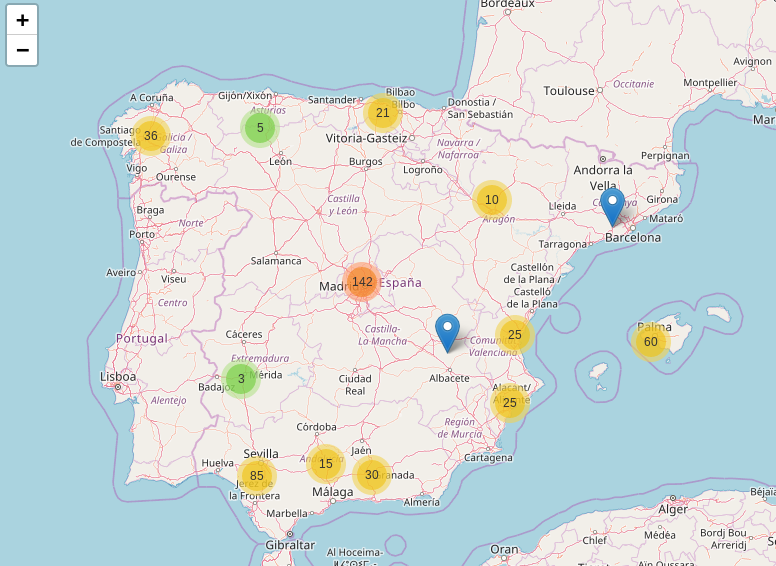
\includegraphics[scale=.50]{Anexos/PuntosNegrosEspana.png}
\caption{Puntos negros de España obtenidos}
\label{blackShapes}
\end{figure}

\begin{figure}[htp]
\centering
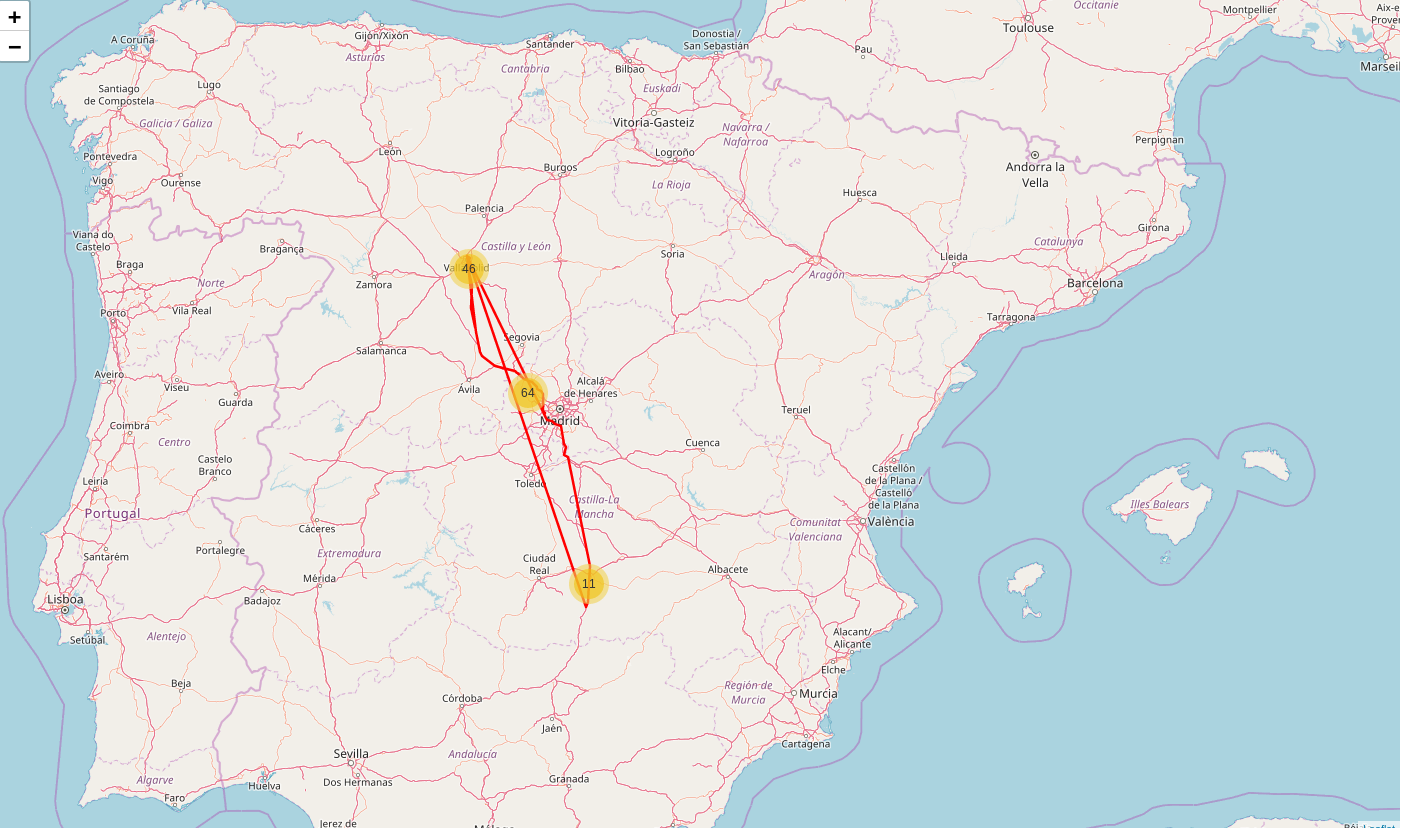
\includegraphics[scale=.30]{Anexos/rutaDeUnVehiculo.png}
\caption{Ruta de un vehiculo}
\label{littleRoute}
\end{figure}


\begin{figure}[htp]
\centering
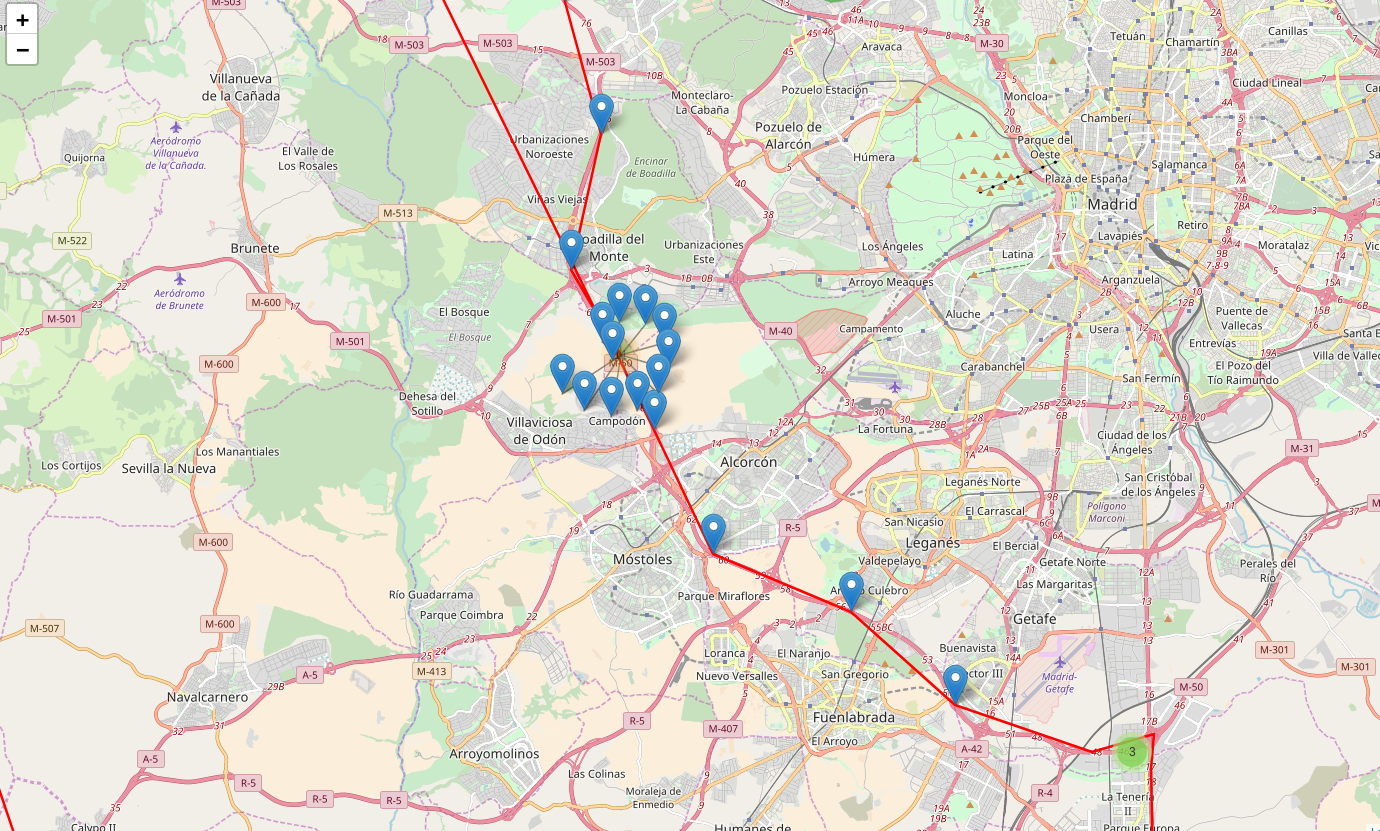
\includegraphics[scale=.30]{Anexos/rutaConParada.png}
\caption{Pequeña ruta y parada de un vehiculo}
\label{littleRouteWithStop}
\end{figure}


\chapter{Script para el API de consultas a MongoDB integrado con OSM}\label{apend.B}
\lstinputlisting[language=Python, basicstyle=\small]{Anexos/mongoUbicationServer.py}

\newpage
\chapter{Script de envio de tramas para la simulación}\label{apend.C}
\lstinputlisting[language=Python, basicstyle=\small]{Anexos/sendTraffic.py}

\newpage
\chapter{Script de SparkSQL Streaming}\label{apend.D}
\lstinputlisting[language=Python, basicstyle=\small]{Anexos/sparkStructStream.py}

\newpage
\chapter{Script de Spark Streaming}\label{apend.E}
\lstinputlisting[language=Python, basicstyle=\small]{Anexos/sparkStreamingWithoutMongo.py}

\newpage
\chapter{Script de SparkSQL Streaming con las consultas a MongoDB}\label{apend.F}
\lstinputlisting[language=Python, basicstyle=\small]{Anexos/sparkStreaming.py}

\newpage
\chapter{Script de creación del índice en Elasticserach}\label{apend.G}
\lstinputlisting[language=Python, basicstyle=\small]{Anexos/CreateIndexForElastic.py}

\newpage
\chapter{Pipe definida para Logstash}\label{apend.H}
\lstinputlisting[basicstyle=\small]{Anexos/logstashkafka.conf}


\newpage
\chapter{Pipe definida para Logstash con actualización}\label{apend.I}
\lstinputlisting[basicstyle=\small]{Anexos/logstashkafkaUpdates.conf}


\newpage
\chapter{Pipe definida para Logstash con actualización}\label{apend.J}
\lstinputlisting[basicstyle=\small]{Anexos/ConsultaTrafico.json}


